% Options for packages loaded elsewhere
\PassOptionsToPackage{unicode}{hyperref}
\PassOptionsToPackage{hyphens}{url}
\PassOptionsToPackage{dvipsnames,svgnames,x11names}{xcolor}
%
\documentclass[
  letterpaper,
  DIV=11,
  numbers=noendperiod]{scrartcl}

\usepackage{amsmath,amssymb}
\usepackage{iftex}
\ifPDFTeX
  \usepackage[T1]{fontenc}
  \usepackage[utf8]{inputenc}
  \usepackage{textcomp} % provide euro and other symbols
\else % if luatex or xetex
  \usepackage{unicode-math}
  \defaultfontfeatures{Scale=MatchLowercase}
  \defaultfontfeatures[\rmfamily]{Ligatures=TeX,Scale=1}
\fi
\usepackage{lmodern}
\ifPDFTeX\else  
    % xetex/luatex font selection
\fi
% Use upquote if available, for straight quotes in verbatim environments
\IfFileExists{upquote.sty}{\usepackage{upquote}}{}
\IfFileExists{microtype.sty}{% use microtype if available
  \usepackage[]{microtype}
  \UseMicrotypeSet[protrusion]{basicmath} % disable protrusion for tt fonts
}{}
\makeatletter
\@ifundefined{KOMAClassName}{% if non-KOMA class
  \IfFileExists{parskip.sty}{%
    \usepackage{parskip}
  }{% else
    \setlength{\parindent}{0pt}
    \setlength{\parskip}{6pt plus 2pt minus 1pt}}
}{% if KOMA class
  \KOMAoptions{parskip=half}}
\makeatother
\usepackage{xcolor}
\setlength{\emergencystretch}{3em} % prevent overfull lines
\setcounter{secnumdepth}{5}
% Make \paragraph and \subparagraph free-standing
\ifx\paragraph\undefined\else
  \let\oldparagraph\paragraph
  \renewcommand{\paragraph}[1]{\oldparagraph{#1}\mbox{}}
\fi
\ifx\subparagraph\undefined\else
  \let\oldsubparagraph\subparagraph
  \renewcommand{\subparagraph}[1]{\oldsubparagraph{#1}\mbox{}}
\fi

\usepackage{color}
\usepackage{fancyvrb}
\newcommand{\VerbBar}{|}
\newcommand{\VERB}{\Verb[commandchars=\\\{\}]}
\DefineVerbatimEnvironment{Highlighting}{Verbatim}{commandchars=\\\{\}}
% Add ',fontsize=\small' for more characters per line
\usepackage{framed}
\definecolor{shadecolor}{RGB}{241,243,245}
\newenvironment{Shaded}{\begin{snugshade}}{\end{snugshade}}
\newcommand{\AlertTok}[1]{\textcolor[rgb]{0.68,0.00,0.00}{#1}}
\newcommand{\AnnotationTok}[1]{\textcolor[rgb]{0.37,0.37,0.37}{#1}}
\newcommand{\AttributeTok}[1]{\textcolor[rgb]{0.40,0.45,0.13}{#1}}
\newcommand{\BaseNTok}[1]{\textcolor[rgb]{0.68,0.00,0.00}{#1}}
\newcommand{\BuiltInTok}[1]{\textcolor[rgb]{0.00,0.23,0.31}{#1}}
\newcommand{\CharTok}[1]{\textcolor[rgb]{0.13,0.47,0.30}{#1}}
\newcommand{\CommentTok}[1]{\textcolor[rgb]{0.37,0.37,0.37}{#1}}
\newcommand{\CommentVarTok}[1]{\textcolor[rgb]{0.37,0.37,0.37}{\textit{#1}}}
\newcommand{\ConstantTok}[1]{\textcolor[rgb]{0.56,0.35,0.01}{#1}}
\newcommand{\ControlFlowTok}[1]{\textcolor[rgb]{0.00,0.23,0.31}{#1}}
\newcommand{\DataTypeTok}[1]{\textcolor[rgb]{0.68,0.00,0.00}{#1}}
\newcommand{\DecValTok}[1]{\textcolor[rgb]{0.68,0.00,0.00}{#1}}
\newcommand{\DocumentationTok}[1]{\textcolor[rgb]{0.37,0.37,0.37}{\textit{#1}}}
\newcommand{\ErrorTok}[1]{\textcolor[rgb]{0.68,0.00,0.00}{#1}}
\newcommand{\ExtensionTok}[1]{\textcolor[rgb]{0.00,0.23,0.31}{#1}}
\newcommand{\FloatTok}[1]{\textcolor[rgb]{0.68,0.00,0.00}{#1}}
\newcommand{\FunctionTok}[1]{\textcolor[rgb]{0.28,0.35,0.67}{#1}}
\newcommand{\ImportTok}[1]{\textcolor[rgb]{0.00,0.46,0.62}{#1}}
\newcommand{\InformationTok}[1]{\textcolor[rgb]{0.37,0.37,0.37}{#1}}
\newcommand{\KeywordTok}[1]{\textcolor[rgb]{0.00,0.23,0.31}{#1}}
\newcommand{\NormalTok}[1]{\textcolor[rgb]{0.00,0.23,0.31}{#1}}
\newcommand{\OperatorTok}[1]{\textcolor[rgb]{0.37,0.37,0.37}{#1}}
\newcommand{\OtherTok}[1]{\textcolor[rgb]{0.00,0.23,0.31}{#1}}
\newcommand{\PreprocessorTok}[1]{\textcolor[rgb]{0.68,0.00,0.00}{#1}}
\newcommand{\RegionMarkerTok}[1]{\textcolor[rgb]{0.00,0.23,0.31}{#1}}
\newcommand{\SpecialCharTok}[1]{\textcolor[rgb]{0.37,0.37,0.37}{#1}}
\newcommand{\SpecialStringTok}[1]{\textcolor[rgb]{0.13,0.47,0.30}{#1}}
\newcommand{\StringTok}[1]{\textcolor[rgb]{0.13,0.47,0.30}{#1}}
\newcommand{\VariableTok}[1]{\textcolor[rgb]{0.07,0.07,0.07}{#1}}
\newcommand{\VerbatimStringTok}[1]{\textcolor[rgb]{0.13,0.47,0.30}{#1}}
\newcommand{\WarningTok}[1]{\textcolor[rgb]{0.37,0.37,0.37}{\textit{#1}}}

\providecommand{\tightlist}{%
  \setlength{\itemsep}{0pt}\setlength{\parskip}{0pt}}\usepackage{longtable,booktabs,array}
\usepackage{calc} % for calculating minipage widths
% Correct order of tables after \paragraph or \subparagraph
\usepackage{etoolbox}
\makeatletter
\patchcmd\longtable{\par}{\if@noskipsec\mbox{}\fi\par}{}{}
\makeatother
% Allow footnotes in longtable head/foot
\IfFileExists{footnotehyper.sty}{\usepackage{footnotehyper}}{\usepackage{footnote}}
\makesavenoteenv{longtable}
\usepackage{graphicx}
\makeatletter
\def\maxwidth{\ifdim\Gin@nat@width>\linewidth\linewidth\else\Gin@nat@width\fi}
\def\maxheight{\ifdim\Gin@nat@height>\textheight\textheight\else\Gin@nat@height\fi}
\makeatother
% Scale images if necessary, so that they will not overflow the page
% margins by default, and it is still possible to overwrite the defaults
% using explicit options in \includegraphics[width, height, ...]{}
\setkeys{Gin}{width=\maxwidth,height=\maxheight,keepaspectratio}
% Set default figure placement to htbp
\makeatletter
\def\fps@figure{htbp}
\makeatother

% load packages
\usepackage{geometry}
\usepackage{xcolor}
\usepackage{eso-pic}
\usepackage{fancyhdr}
\usepackage{sectsty}
\usepackage{fontspec}
\usepackage{titlesec}

%% Set page size with a wider right margin
\geometry{a4paper, total={170mm,257mm}, left=20mm, top=20mm, bottom=20mm, right=50mm}

%% Let's define some colours
\definecolor{uniblue}{HTML}{003865}
\definecolor{burgundy}{HTML}{7D2239}
\definecolor{cobalt}{HTML}{005C8A}
\definecolor{lavender}{HTML}{5B4D94}
\definecolor{leaf}{HTML}{006630}
\definecolor{moss}{HTML}{385A4F}
\definecolor{pillarbox}{HTML}{B30C00}
\definecolor{rust}{HTML}{9A3A06}
\definecolor{sandstone}{HTML}{52473B}
\definecolor{skyblue}{HTML}{005398}
\definecolor{slate}{HTML}{4F5961}
\definecolor{thistle}{HTML}{951272}

%\definecolor{light}{HTML}{E6E6FA} % original from template - redefined below as uni blue at 10 percent:
\colorlet{light}{uniblue!10}
%\definecolor{highlight}{HTML}{800080} % original from template - redefined below as uni's skyblue:
\colorlet{highlight}{skyblue}
%\definecolor{dark}{HTML}{330033} % original from template - redefined below as uni blue at 100 percent:
\colorlet{dark}{uniblue}

%% Let's add the border on the right hand side 
\AddToShipoutPicture{% 
    \AtPageLowerLeft{% 
        \put(\LenToUnit{\dimexpr\paperwidth-3cm},0){% 
            \color{light}\rule{3cm}{\LenToUnit\paperheight}%
          }%
     }%
     % logo
    \AtPageLowerLeft{% start the bar at the bottom right of the page
        \put(\LenToUnit{\dimexpr\paperwidth-2.25cm},27.2cm){% move it to the top right
            \color{light}
\includegraphics[width=2.25cm]{_extensions/nrennie/PrettyPDF/uni_logo_boxed.jpg}
          }%
     }%
}

%% Style the page number
\fancypagestyle{mystyle}{
  \fancyhf{}
  \renewcommand\headrulewidth{0pt}
  \fancyfoot[R]{\thepage}
  \fancyfootoffset{3.5cm}
}
\setlength{\footskip}{20pt}

%% style the chapter/section fonts
\chapterfont{\color{uniblue}\fontsize{20}{16.8}\selectfont}
\sectionfont{\color{uniblue}\fontsize{20}{16.8}\selectfont}
\subsectionfont{\color{skyblue}\fontsize{14}{16.8}\selectfont}
\titleformat{\subsection}
  {\color{uniblue!90}\sffamily\Large\bfseries}{\thesubsection}{1em}{}[{\titlerule[0.8pt]}]
\subsubsectionfont{\color{cobalt}}

\renewcommand\thesection{\color{slate}\arabic{section}}
  
% left align title
\makeatletter
\renewcommand{\maketitle}{\bgroup\setlength{\parindent}{0pt}
\begin{flushleft}
  {\color{uniblue}\sffamily\huge\textbf{\@title}} \vspace{0.3cm} \newline
  {\Large {\@subtitle}} \newline
  \@author
\end{flushleft}\egroup
}
\makeatother

%% Use some custom fonts
\setsansfont{Ubuntu}[
    Path=_extensions/nrennie/PrettyPDF/Ubuntu/,
    Scale=0.9,
    Extension = .ttf,
    UprightFont=*-Regular,
    BoldFont=*-Bold,
    ItalicFont=*-Italic,
    ]

\setmainfont{Ubuntu}[
    Path=_extensions/nrennie/PrettyPDF/Ubuntu/,
    Scale=0.9,
    Extension = .ttf,
    UprightFont=*-Regular,
    BoldFont=*-Bold,
    ItalicFont=*-Italic,
    ]
\KOMAoption{captions}{tableheading}
\makeatletter
\@ifpackageloaded{tcolorbox}{}{\usepackage[skins,breakable]{tcolorbox}}
\@ifpackageloaded{fontawesome5}{}{\usepackage{fontawesome5}}
\definecolor{quarto-callout-color}{HTML}{909090}
\definecolor{quarto-callout-note-color}{HTML}{0758E5}
\definecolor{quarto-callout-important-color}{HTML}{CC1914}
\definecolor{quarto-callout-warning-color}{HTML}{EB9113}
\definecolor{quarto-callout-tip-color}{HTML}{00A047}
\definecolor{quarto-callout-caution-color}{HTML}{FC5300}
\definecolor{quarto-callout-color-frame}{HTML}{acacac}
\definecolor{quarto-callout-note-color-frame}{HTML}{4582ec}
\definecolor{quarto-callout-important-color-frame}{HTML}{d9534f}
\definecolor{quarto-callout-warning-color-frame}{HTML}{f0ad4e}
\definecolor{quarto-callout-tip-color-frame}{HTML}{02b875}
\definecolor{quarto-callout-caution-color-frame}{HTML}{fd7e14}
\makeatother
\makeatletter
\@ifpackageloaded{caption}{}{\usepackage{caption}}
\AtBeginDocument{%
\ifdefined\contentsname
  \renewcommand*\contentsname{Table of contents}
\else
  \newcommand\contentsname{Table of contents}
\fi
\ifdefined\listfigurename
  \renewcommand*\listfigurename{List of Figures}
\else
  \newcommand\listfigurename{List of Figures}
\fi
\ifdefined\listtablename
  \renewcommand*\listtablename{List of Tables}
\else
  \newcommand\listtablename{List of Tables}
\fi
\ifdefined\figurename
  \renewcommand*\figurename{Figure}
\else
  \newcommand\figurename{Figure}
\fi
\ifdefined\tablename
  \renewcommand*\tablename{Table}
\else
  \newcommand\tablename{Table}
\fi
}
\@ifpackageloaded{float}{}{\usepackage{float}}
\floatstyle{ruled}
\@ifundefined{c@chapter}{\newfloat{codelisting}{h}{lop}}{\newfloat{codelisting}{h}{lop}[chapter]}
\floatname{codelisting}{Listing}
\newcommand*\listoflistings{\listof{codelisting}{List of Listings}}
\makeatother
\makeatletter
\makeatother
\makeatletter
\@ifpackageloaded{caption}{}{\usepackage{caption}}
\@ifpackageloaded{subcaption}{}{\usepackage{subcaption}}
\makeatother
\makeatletter
\@ifpackageloaded{tcolorbox}{}{\usepackage[skins,breakable]{tcolorbox}}
\makeatother
\makeatletter
\@ifundefined{shadecolor}{\definecolor{shadecolor}{rgb}{.97, .97, .97}}{}
\makeatother
\makeatletter
\@ifundefined{codebgcolor}{\definecolor{codebgcolor}{named}{light}}{}
\makeatother
\makeatletter
\ifdefined\Shaded\renewenvironment{Shaded}{\begin{tcolorbox}[frame hidden, boxrule=0pt, colback={codebgcolor}, sharp corners, enhanced, breakable]}{\end{tcolorbox}}\fi
\makeatother
\ifLuaTeX
  \usepackage{selnolig}  % disable illegal ligatures
\fi
\usepackage{bookmark}

\IfFileExists{xurl.sty}{\usepackage{xurl}}{} % add URL line breaks if available
\urlstyle{same} % disable monospaced font for URLs
\hypersetup{
  pdftitle={Authoring presentations with Quarto},
  colorlinks=true,
  linkcolor={highlight},
  filecolor={Maroon},
  citecolor={Blue},
  urlcolor={highlight},
  pdfcreator={LaTeX via pandoc}}

\title{Authoring presentations with Quarto}
\author{}
\date{}

\begin{document}
\maketitle

\pagestyle{mystyle}

\section{Quarto Presentations}\label{quarto-presentations}

Another great feature of Quarto is that it allows you to create
presentations and supports a variety of formats such as
\href{https://quarto.org/docs/presentations/revealjs/}{html},
\href{https://quarto.org/docs/presentations/powerpoint.html}{power
point} and
\href{https://quarto.org/docs/presentations/beamer.html}{beamer}. Today
we will focus on creating an html presentation (which can be also
printed as a pdf).

Creating an html presentation is as easy as setting the output format to
\texttt{revealjs}:

\begin{Shaded}
\begin{Highlighting}[]

\SpecialCharTok{{-}{-}{-}}

\NormalTok{title}\SpecialCharTok{:} \StringTok{"My title"}

\NormalTok{author}\SpecialCharTok{:} \StringTok{"Jafet Belmont"}

\NormalTok{format}\SpecialCharTok{:}\NormalTok{ revealjs}

\SpecialCharTok{{-}{-}{-}}
\end{Highlighting}
\end{Shaded}

This will create a title slide that includes the provided \texttt{title}
and \texttt{author}. (you can remove any of these options if you the
author or title page to be removed). Now we will switch to the
\texttt{visual} mode. You will notice that a new set of options have now
appeared:

\begin{center}
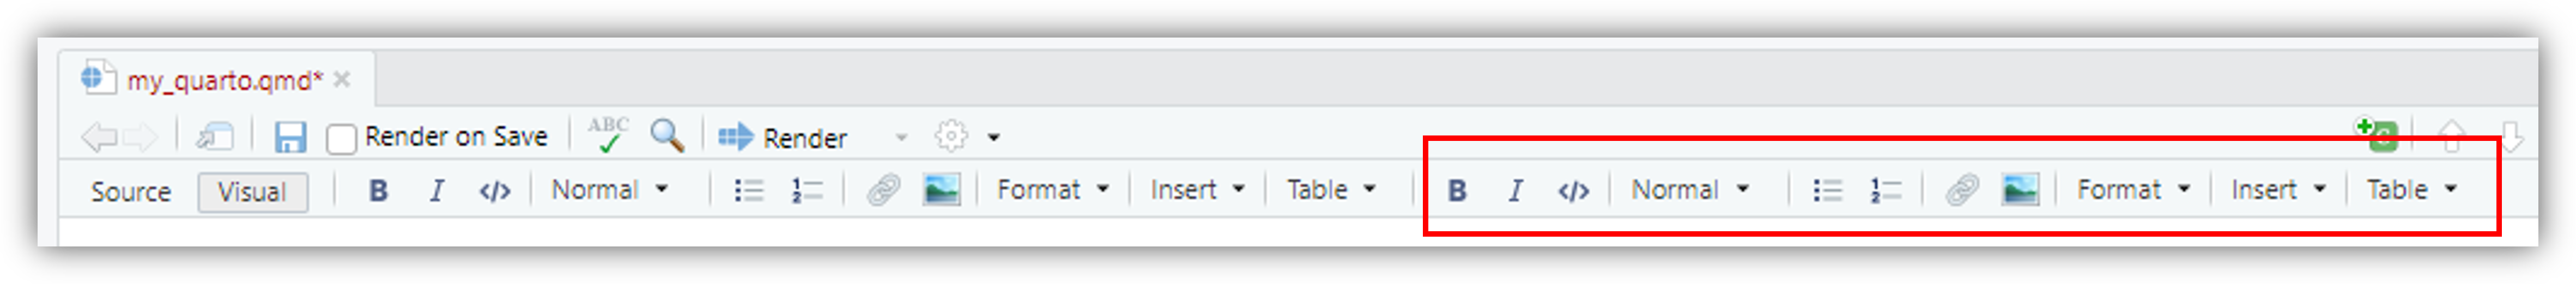
\includegraphics{images/quarto13.png}
\end{center}

This new tab will allow us to interact with the different features of
our presentation. Lets begin by creating some slides. Slides in Quarto
are delineated using level 1 and 2 headings:

\begin{Shaded}
\begin{Highlighting}[]

\SpecialCharTok{{-}{-}{-}}

\NormalTok{title}\SpecialCharTok{:} \StringTok{"My title"}

\NormalTok{author}\SpecialCharTok{:} \StringTok{"Jafet Belmont"}

\NormalTok{format}\SpecialCharTok{:}\NormalTok{ revealjs}

\SpecialCharTok{{-}{-}{-}}

\CommentTok{\# Topic 1}

\DocumentationTok{\#\# Slide 1.1}

\CommentTok{\# Topic 2}

\DocumentationTok{\#\# Slide 2.1}
\end{Highlighting}
\end{Shaded}

In the example above we use level 1 headings for creating a new sections
and level 2 heading for defining the new slides. Alternatively we can
use horizontal rules to create the slides as follows (on \texttt{visual}
mode click on \texttt{Insert▾\ ➠\ Horizontal\ Rule}):

\begin{Shaded}
\begin{Highlighting}[]

\SpecialCharTok{{-}{-}{-}}

\NormalTok{title}\SpecialCharTok{:} \StringTok{"My title"}

\NormalTok{author}\SpecialCharTok{:} \StringTok{"Jafet Belmont"}

\NormalTok{format}\SpecialCharTok{:}\NormalTok{ revealjs}

\SpecialCharTok{{-}{-}{-}}

\NormalTok{  Content of slide }\DecValTok{1}

\SpecialCharTok{{-}{-}{-}}

\NormalTok{  Content of slide }\DecValTok{2}

\SpecialCharTok{{-}{-}{-}}
\end{Highlighting}
\end{Shaded}

You can add bullet and numbered lists to each slide as follows (on
\texttt{visual} mode click on

\includegraphics[width=0.25in,height=0.26042in]{images/bullets.png} or

\includegraphics[width=0.3125in,height=0.26042in]{images/numbered.png}
for adding bullet or numbered lists respectively):

\begin{Shaded}
\begin{Highlighting}[]

\SpecialCharTok{{-}{-}{-}}

\NormalTok{title}\SpecialCharTok{:} \StringTok{"My title"}

\NormalTok{author}\SpecialCharTok{:} \StringTok{"Jafet Belmont"}

\NormalTok{format}\SpecialCharTok{:}\NormalTok{ revealjs}

\SpecialCharTok{{-}{-}{-}}

\DocumentationTok{\#\# Slide 1}

\FloatTok{1.}\NormalTok{  Item }\DecValTok{1}

\FloatTok{2.}\NormalTok{  Item }\DecValTok{2}

\DocumentationTok{\#\# Slide 2}

\SpecialCharTok{{-}}\NormalTok{   Bullet }\DecValTok{1}

    \SpecialCharTok{{-}}\NormalTok{   Bullet }\FloatTok{1.1}

    \SpecialCharTok{{-}}\NormalTok{   Bullet }\FloatTok{1.2}

\SpecialCharTok{{-}}\NormalTok{   Bulet }\DecValTok{2}

    \SpecialCharTok{{-}}\NormalTok{   Bullet }\FloatTok{2.1}

    \SpecialCharTok{{-}}\NormalTok{   Bullet }\FloatTok{2.2}
\end{Highlighting}
\end{Shaded}

Notice that indentation allow us to create a hierarchical structure
within our lists of items. You can modify some of the option of the list
by clicking the

\includegraphics[width=0.15625in,height=\textheight]{images/threedots.png}
button on the right side of it. This will open a pop-up window where you
can modify some of its attributes. For example, you can ask Quarto to
display each item one by one as you move forward through the slides:

\begin{center}
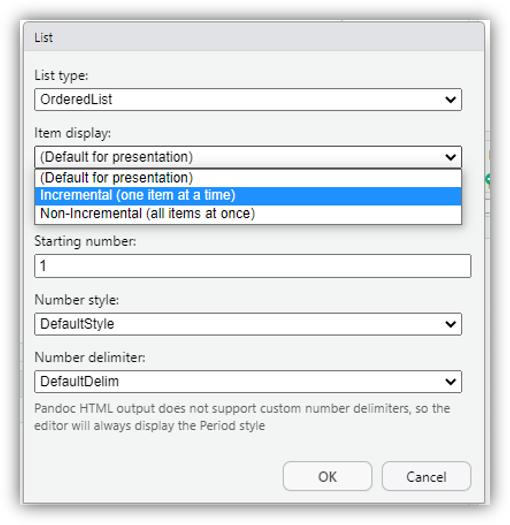
\includegraphics[width=3.8125in,height=\textheight]{images/quarto11.png}
\end{center}

If you want to arrange the content of you slide into different columns
you can insert a multiple column output. To do this switch to
\texttt{visual} mode and click on \texttt{Insert▾\ ➠\ Slide\ Columns}).
You can then fill each column:

\begin{center}
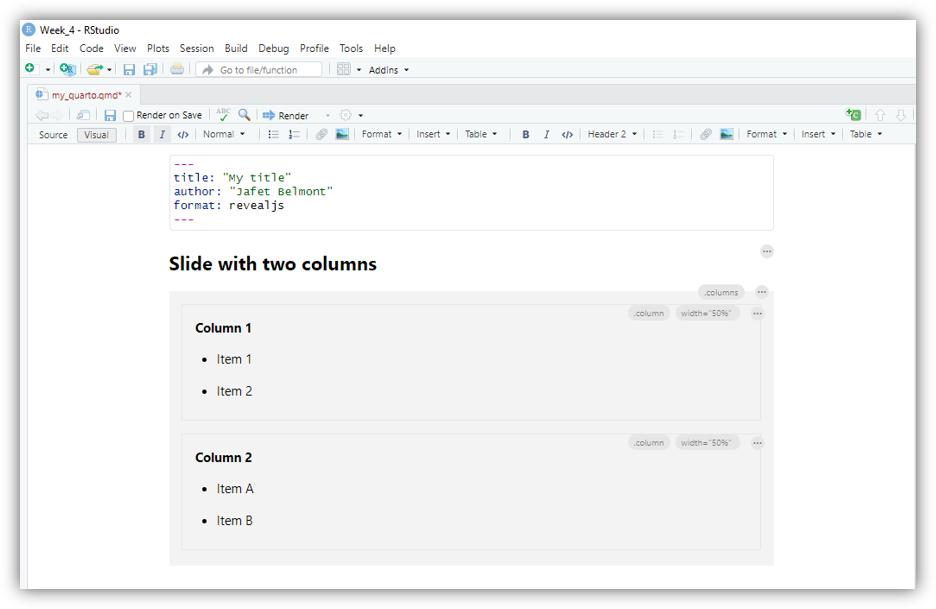
\includegraphics{images/quarto12.png}
\end{center}

Sometimes the text size in your slide might be too large to fit in your
slide and you would like to make it smaller. You can then use the
.smaller class to use a smaller typeface so that more text fits on the
slide.

\begin{Shaded}
\begin{Highlighting}[]

\SpecialCharTok{{-}{-}{-}}

\NormalTok{title}\SpecialCharTok{:} \StringTok{"My title"}

\NormalTok{author}\SpecialCharTok{:} \StringTok{"Jafet Belmont"}

\NormalTok{format}\SpecialCharTok{:}\NormalTok{ revealjs}

\SpecialCharTok{{-}{-}{-}}

\DocumentationTok{\#\# Slide with small text \{.smaller\}}

\FloatTok{1.}\NormalTok{  Item }\DecValTok{1}

\FloatTok{2.}\NormalTok{  Item }\DecValTok{2}

 
\end{Highlighting}
\end{Shaded}

~If you are on the visual model, click on the slide settings

\includegraphics[width=0.17708in,height=\textheight]{images/threedots.png}
and then type \texttt{.smaller} on the class box:

\begin{center}
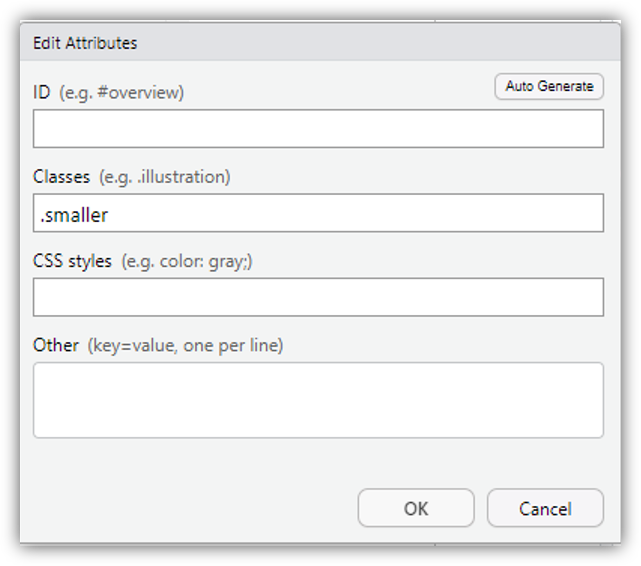
\includegraphics[width=3.88542in,height=\textheight]{images/quarto14.png}
\end{center}

\begin{tcolorbox}[enhanced jigsaw, colframe=quarto-callout-note-color-frame, bottomtitle=1mm, breakable, coltitle=black, colbacktitle=quarto-callout-note-color!10!white, opacityback=0, rightrule=.15mm, titlerule=0mm, title=\textcolor{quarto-callout-note-color}{\faInfo}\hspace{0.5em}{Note}, toprule=.15mm, colback=white, left=2mm, opacitybacktitle=0.6, bottomrule=.15mm, arc=.35mm, toptitle=1mm, leftrule=.75mm]

Note that ideally you slides should not contain too much text and thus
this is just a quick way around if you feel that you need a bit of extra
space in your slide.

\end{tcolorbox}

R code can be embedded in any slides by including a R chunk in the same
way as we did before. However, sometimes we would like to arrange the
code output to be display in a ``tidy'' manner within the slide. To
achieve this we can use the \texttt{output-location:} argument which has
the following options:

\begin{itemize}
\item
  \texttt{column}: Display output in a column adjacent to the code
\item
  \texttt{column-fragment}: Display output in a column adjacent to the
  code and delay showing it until its explicitly stepped through by
  advancing the slides.
\item
  \texttt{fragment}: Delay the output display until it is explicitly
  stepped through by advancing the slides.
\item
  \texttt{slide}: Display output on the subsequent slide.

  For example, the source code for a chunk within a slide containing an
  R code would look something like this:

\begin{Shaded}
\begin{Highlighting}[]

\CommentTok{\#| output{-}location: column{-}fragment}

\FunctionTok{ggplot}\NormalTok{(evals.scores, }\FunctionTok{aes}\NormalTok{(}\AttributeTok{x =}\NormalTok{ bty\_avg, }\AttributeTok{y =}\NormalTok{ score)) }\SpecialCharTok{+}

  \FunctionTok{geom\_point}\NormalTok{() }\SpecialCharTok{+}

  \FunctionTok{labs}\NormalTok{(}\AttributeTok{x =} \StringTok{"Beauty Score"}\NormalTok{, }\AttributeTok{y =} \StringTok{"Teaching Score"}\NormalTok{) }\SpecialCharTok{+}

  \FunctionTok{geom\_smooth}\NormalTok{(}\AttributeTok{method =} \StringTok{"lm"}\NormalTok{, }\AttributeTok{se =} \ConstantTok{FALSE}\NormalTok{)}
\end{Highlighting}
\end{Shaded}
\end{itemize}



\end{document}
